\chapter{Kinematics}\label{c:K}

\section{Specific Jet Feature Distributions}

	For the standard set of jet features, plot the overall distributions in a standard 2 hist ratio plot for data and MC. This also includes jet counts possibly


\section{Specific Jet Feature Distributions}

	\subsection{Two Central Channel}
	
		\begin{itemize}
			\item $b$-jet1
			\item $b$-jet2
			\item F-jet
			\item jet
		\end{itemize}
		
		For each of these jets, which we can define, plot standard kinematic variables, \pt, $\eta$, $\phi$, m. Torn as to the options here. could do more 2d jet to jet ratio plots, could do a more general distribution ratio for each one, and then there is s/b to consider. Could argue jet to jet comparisons moot as we already covered that.

\section{BDT Input Variables}

	\begin{itemize}
		\item $M_{jj}$
		\item \pt$_{jj}$
		\item $\cos \theta$
		\item $\Delta\eta_{jj}$
		\item $Max(\eta)$
		\item $\eta*$
		\item $min\Delta R(j_1)$
		\item $min\Delta R(j_1)$
		\item \pt balance
		\item $N_{TRK}(j_1) PV500$ ?
		\item $N_{TRK}(j_) PV500$ ?
	\end{itemize}
	
		\begin{figure}[h]
			\centering
			
			\begin{minipage}[h]{0.33\linewidth}
				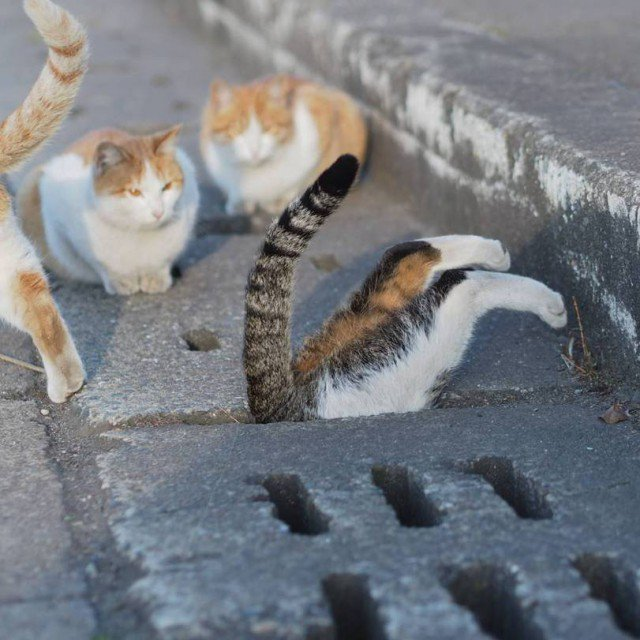
\includegraphics[width=1\linewidth]{placeholder}
			\end{minipage}
			\quad
			\begin{minipage}[h]{0.33\linewidth}
				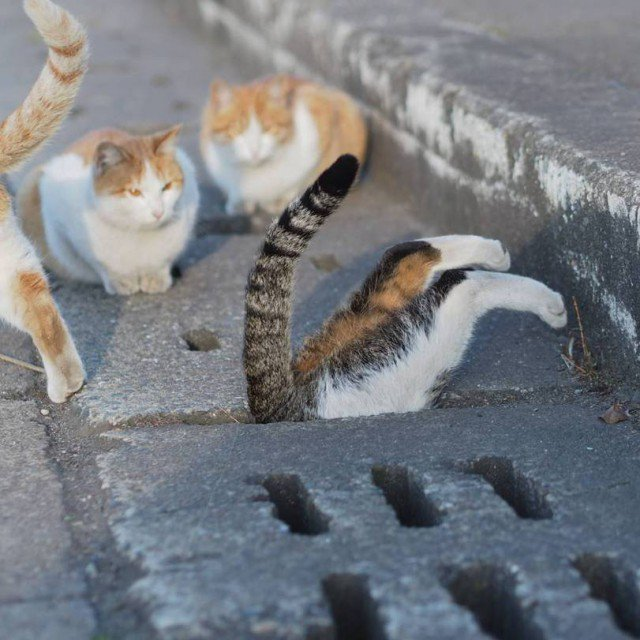
\includegraphics[width=1\linewidth]{placeholder}
			\end{minipage}
			\caption{For Each channel, a standard 2 hist ratio plot fo the values of the BDT variables mentioned above, i.e. offline hist and online hists with a ratio. Each plot would have 4 lines, background(data) on/off, signal(MC) on/off and two ratios: data on/off + Mc on/off}
				\label{fig:bdtmjj}
		\end{figure}


\section{Mbb Distribution}

	Prior paper suggests this is the 'final' plot, a shape comparison between BDT influenced control and signal regions of the Mbb distribution. A little confused as to exactly what we need here.

\endinput
